
\documentclass{beamer}


\mode<presentation>
{
  \usetheme{Singapore}
  \renewcommand{\insertnavigation}[1]{}
  \setbeamercovered{transparent}
}



\usepackage[english]{babel}
\usepackage[absolute,overlay]{textpos}
\usepackage[latin1]{inputenc}
\usepackage{times}
\usepackage{graphicx}
\usepackage{epstopdf}
\usepackage[T1]{fontenc}
\usepackage{soul}
\usepackage{pdflscape}
\usepackage{multirow}

\beamertemplatenavigationsymbolsempty

\newcommand{\citations}[1]
   {
     \begin{textblock}{16}[1,1](15.75,15.25)
       \flushright{\scriptsize #1}
     \end{textblock}
   }

\definecolor{MedPurple}{RGB}{194,165,207}
\definecolor{DeepPurple}{RGB}{118,42,131}
\definecolor{LightGreen}{RGB}{166,219,160}
\definecolor{DarkGreen}{RGB}{0,68,27}
\definecolor{MedGreen}{RGB}{90,174,97}

\setbeamercolor{title}{fg=DeepPurple}
\setbeamercolor{frametitle}{fg=DeepPurple}
\setbeamercolor{structure}{fg=DarkGreen}

\setbeamercolor{*}{bg=LightGreen}

\title[Specialisation \& the Latitude-niche-breadth Hypothesis]
{Specialisation \& the Latitude-niche-breadth Hypothesis}

\author[A.R. Cirtwill, D.B. Stouffer, \& T.N. Romanuk]{\textbf{Alyssa R. Cirtwill}, Daniel B. Stouffer, \& Tamara N. Romanuk} 
\institute[]
{
 %
  Stouffer Lab\\
  School of Biological Sciences\\
  University of Canterbury\\
  Christchurch, New Zealand\\
  ~\\
  www.stoufferlab.org\\
  %
}
\date[Short Occasion] 
{23 October 2015 | ABC 2015}

\subject{Talks}

\begin{document}

% \begin{frame}
%   \titlepage
% \end{frame}

% %%Start Introduction Slides%%
\section*{Background}

  \begin{frame}{Why are there more species in the tropics?}

    \begin{center}
      \includegraphics*[width=.8\textwidth]{Figures/plant_richness.eps}

      \vspace{1cm}

    \textbf{Alyssa R. Cirtwill}, Daniel B. Stouffer, Tamara N. Romanuk

    \vspace{1cm}

    23 October 2015 | ABC 2015

    \end{center}
  \end{frame}


  \begin{frame}{Why are there more species in the tropics?}

    \begin{center}
      \includegraphics*[width=.8\textwidth]{Figures/plant_richness.eps}

      \vspace{1cm}

      Envionmental stability? 
      Productivity? 
      Speciation rates?

      \vspace{1cm}
      {\color{white} 23 October 2015 | ABC 2015}
    \end{center}
  \end{frame}


  \begin{frame}{Why are there more species in the tropics?}

    \begin{center}
      \includegraphics*[width=.8\textwidth]{Figures/plant_richness.eps}


      \vspace{1cm}

      \textbf{Envionmental stability?} 
      \textbf{Productivity?} 
      Speciation rates?

      \vspace{1cm}
      {\color{white} 23 October 2015 | ABC 2015}

    \end{center}
  \end{frame}


  \begin{frame}{Latitude-Niche Breadth Hypothesis}

    \begin{center}
      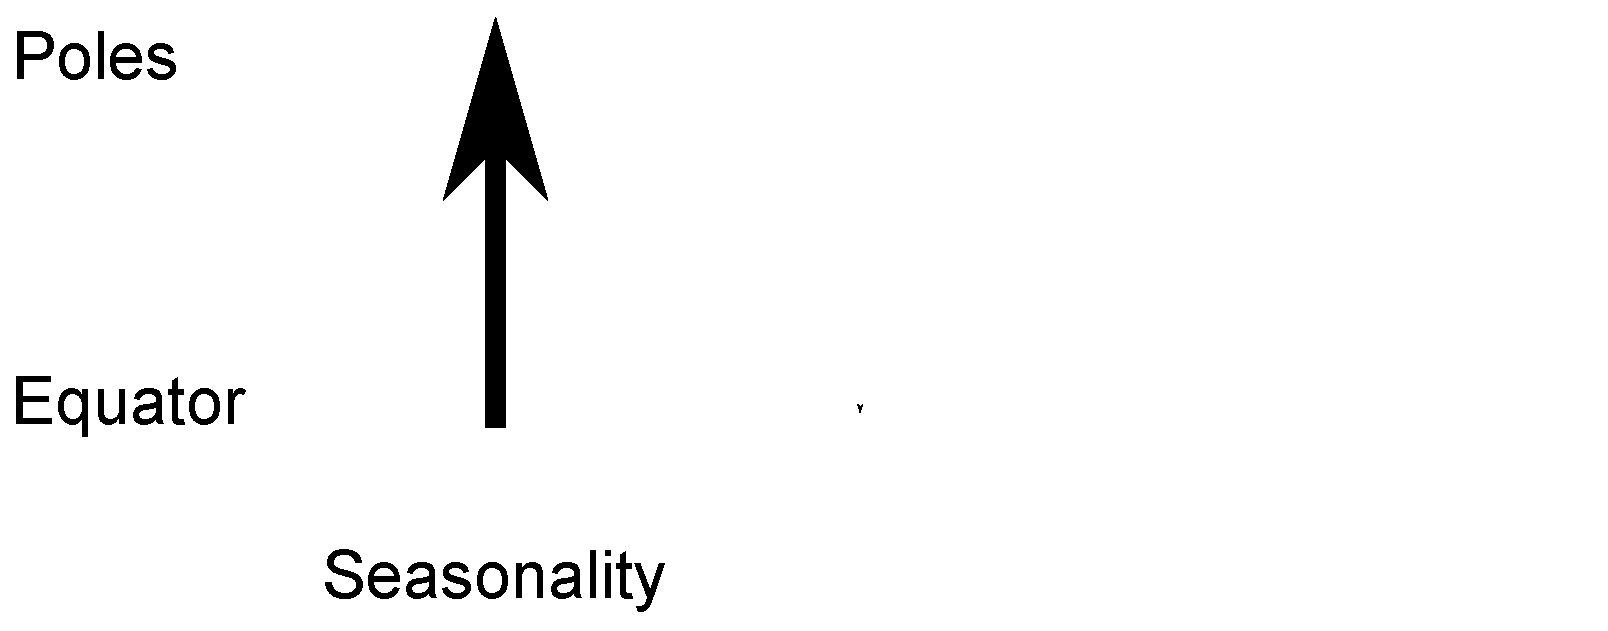
\includegraphics[width=.8\textwidth]{Figures/latitude_niche_breadth_1.eps}
    \end{center}

    \footnotesize{Vazquez, D.P. \& Stevens, R.D. 2004. The latitudinal gradient in niche breadth: concepts and evidence. \emph{The American Naturalist} \textbf{164}, E1-19.}
  \end{frame}


  \begin{frame}{Latitude-Niche Breadth Hypothesis}

    \begin{center}
      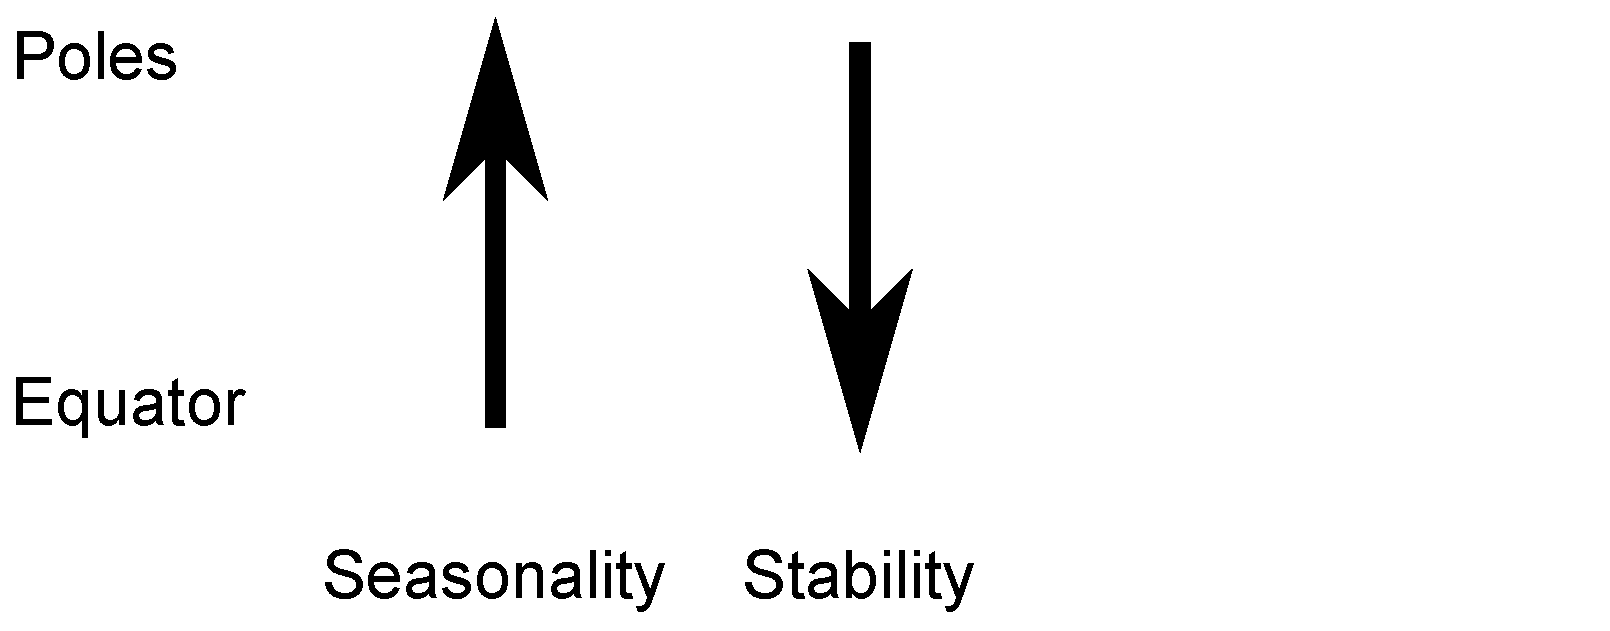
\includegraphics[width=.8\textwidth]{Figures/latitude_niche_breadth_2.eps}
    \end{center}

    \footnotesize{Vazquez, D.P. \& Stevens, R.D. 2004. The latitudinal gradient in niche breadth: concepts and evidence. \emph{The American Naturalist} \textbf{164}, E1-19.}
  \end{frame}


  \begin{frame}{Latitude-Niche Breadth Hypothesis}

    \begin{center}
      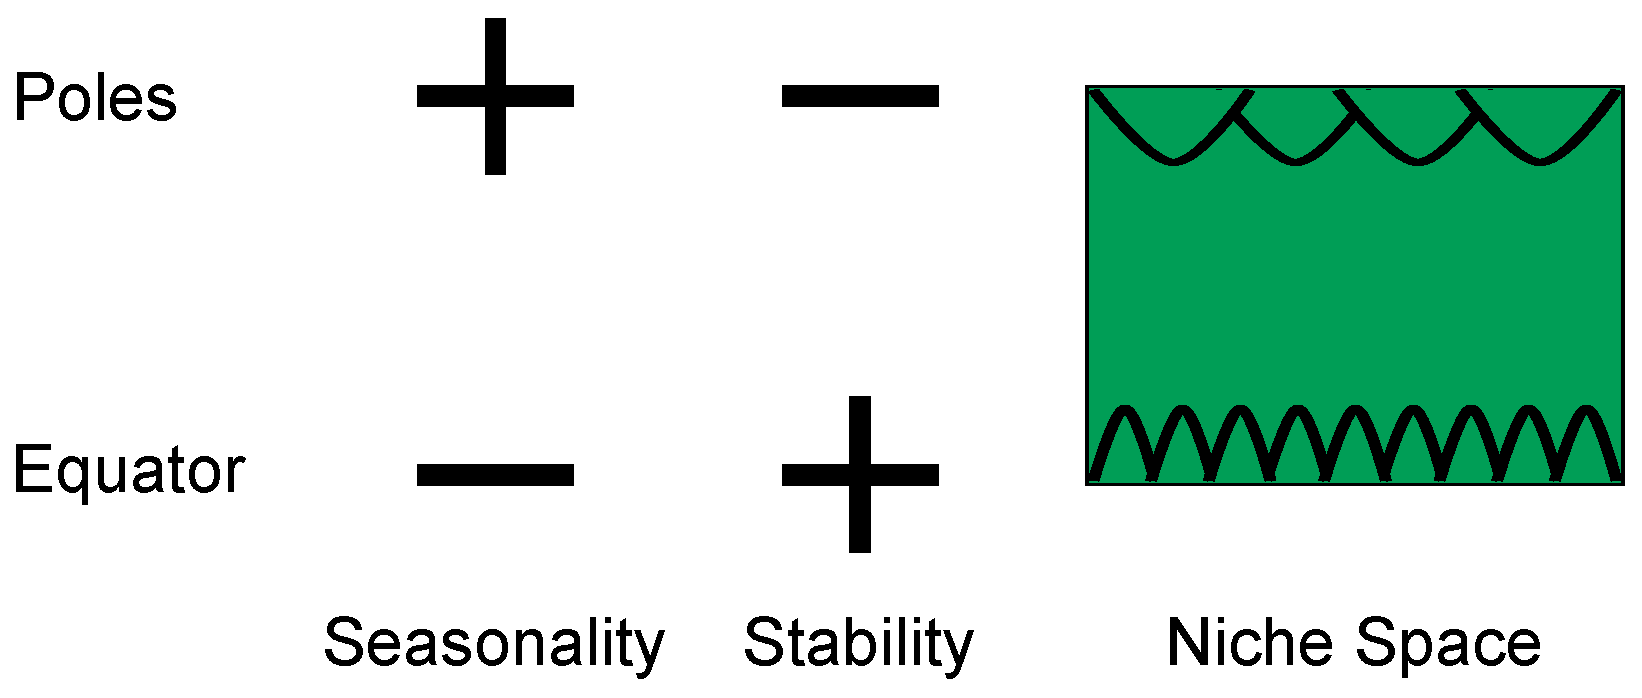
\includegraphics[width=.8\textwidth]{Figures/latitude_niche_breadth_3.eps}
    \end{center}

    \footnotesize{Vazquez, D.P. \& Stevens, R.D. 2004. The latitudinal gradient in niche breadth: concepts and evidence. \emph{The American Naturalist} \textbf{164}, E1-19.}
  \end{frame}


  \begin{frame}{Alternatively ...}

    \begin{center}
      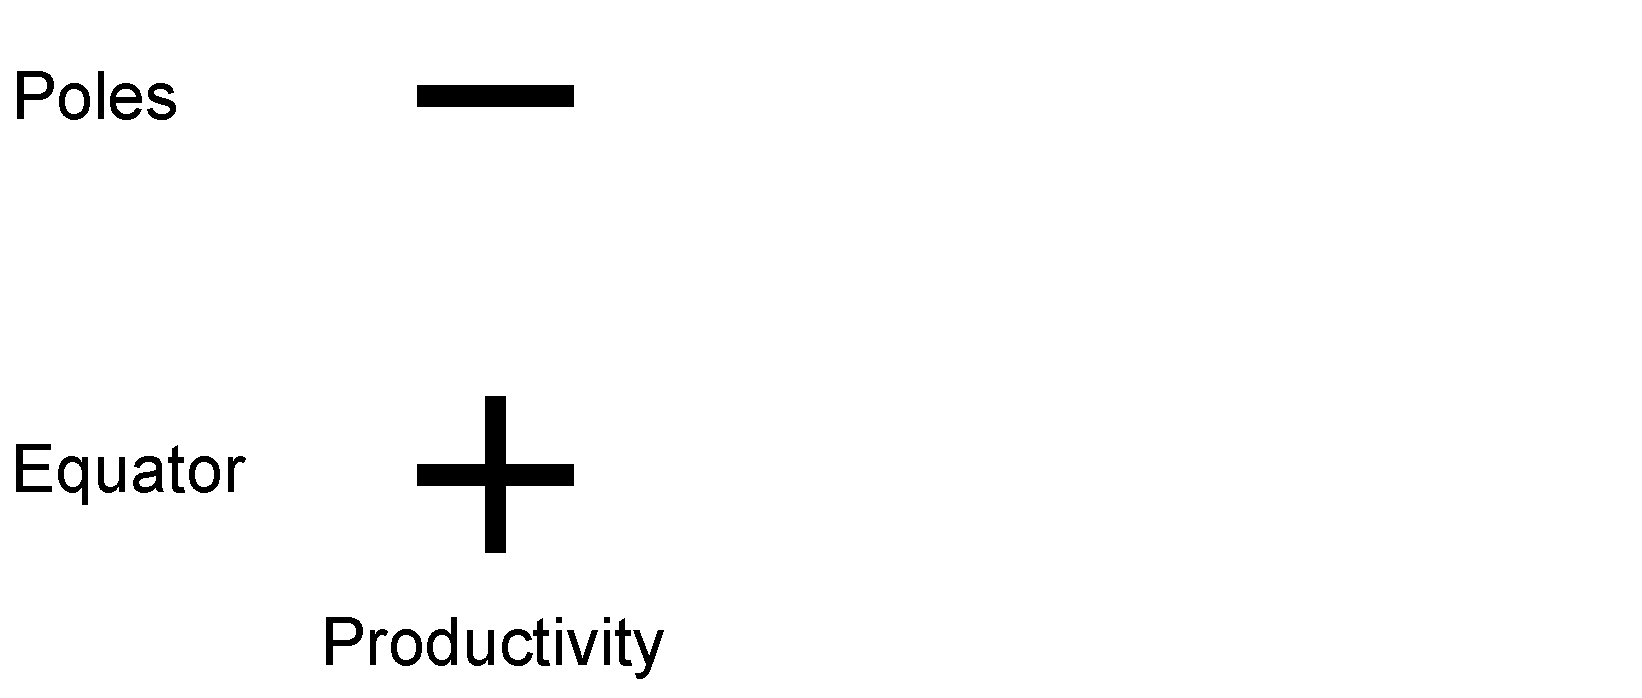
\includegraphics[width=.8\textwidth]{Figures/latitude_niche_breadth_4.eps}
    \end{center}

    \tiny{Davies \emph{et. al.} 2007. Productivity alters the scale dependence of the diversity-invasibility relationship. \emph{Ecology} \textbf{88}, 1940-1947.}
  \end{frame}


  \begin{frame}{Alternatively ...}

    \begin{center}
      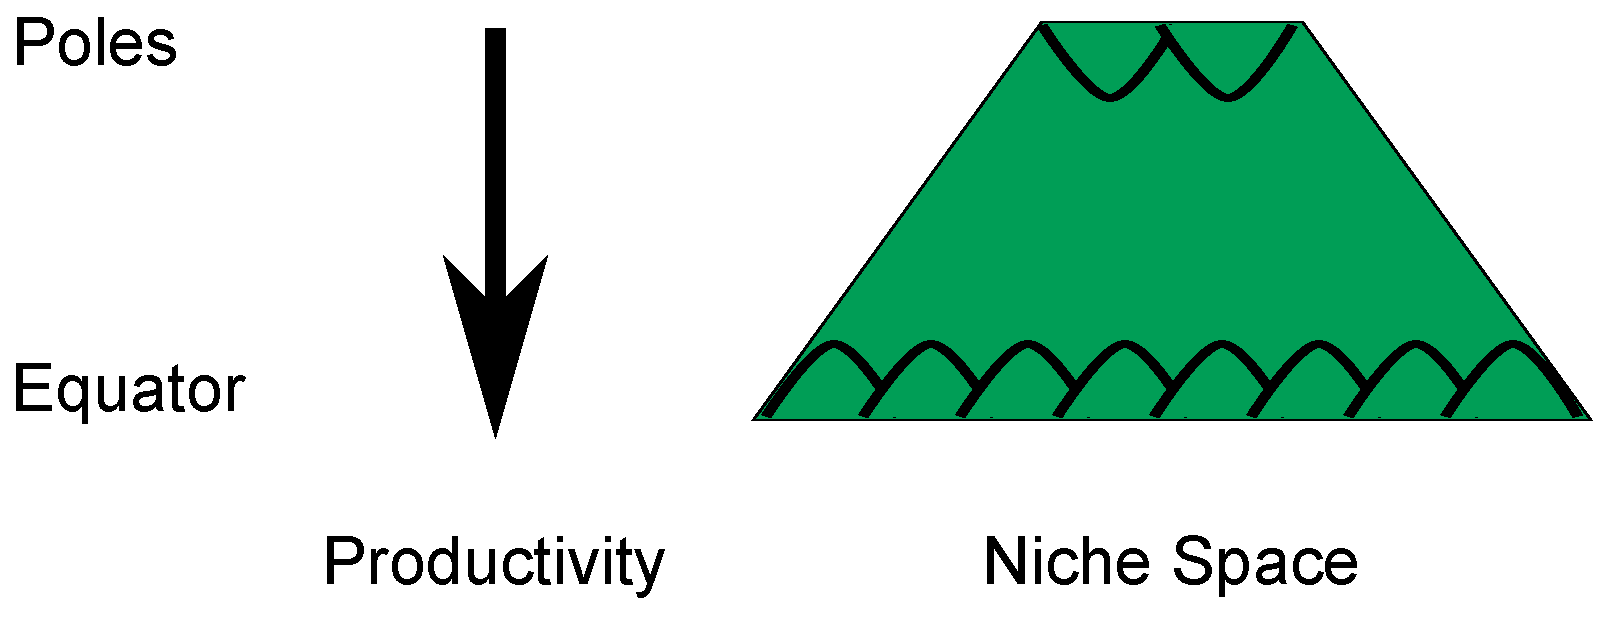
\includegraphics[width=.8\textwidth]{Figures/latitude_niche_breadth_5.eps}
    \end{center}

    \tiny{Davies \emph{et. al.} 2007. Productivity alters the scale dependence of the diversity-invasibility relationship. \emph{Ecology} \textbf{88}, 1940-1947.}
  \end{frame}


\section*{Food Webs}
  \begin{frame}{Testing The Hypotheses}

    \begin{center}
      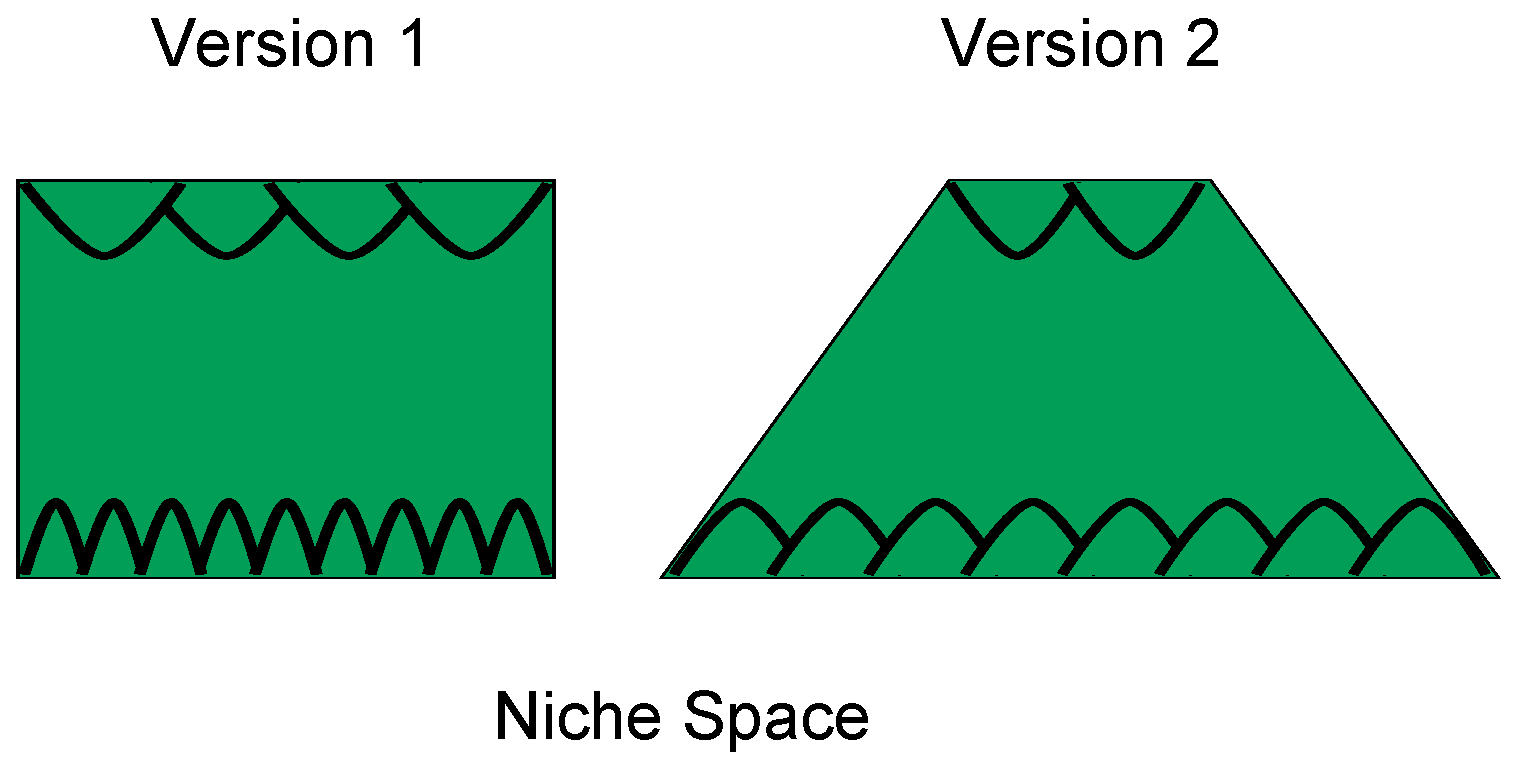
\includegraphics[width=.8\textwidth]{Figures/hypothesis_comparison.eps}

    \end{center}

    \begin{columns}
    \column{.5in}
    \column{1.75in}
      - Greater specialisation in the tropics
    \column{.5in}
    \column{1.75in}
      - Similar specialisation at all latitudes
    \column{.5in}
    \end{columns}

  \end{frame}


  \begin{frame}{Testing The Hypotheses}

    \begin{center}
      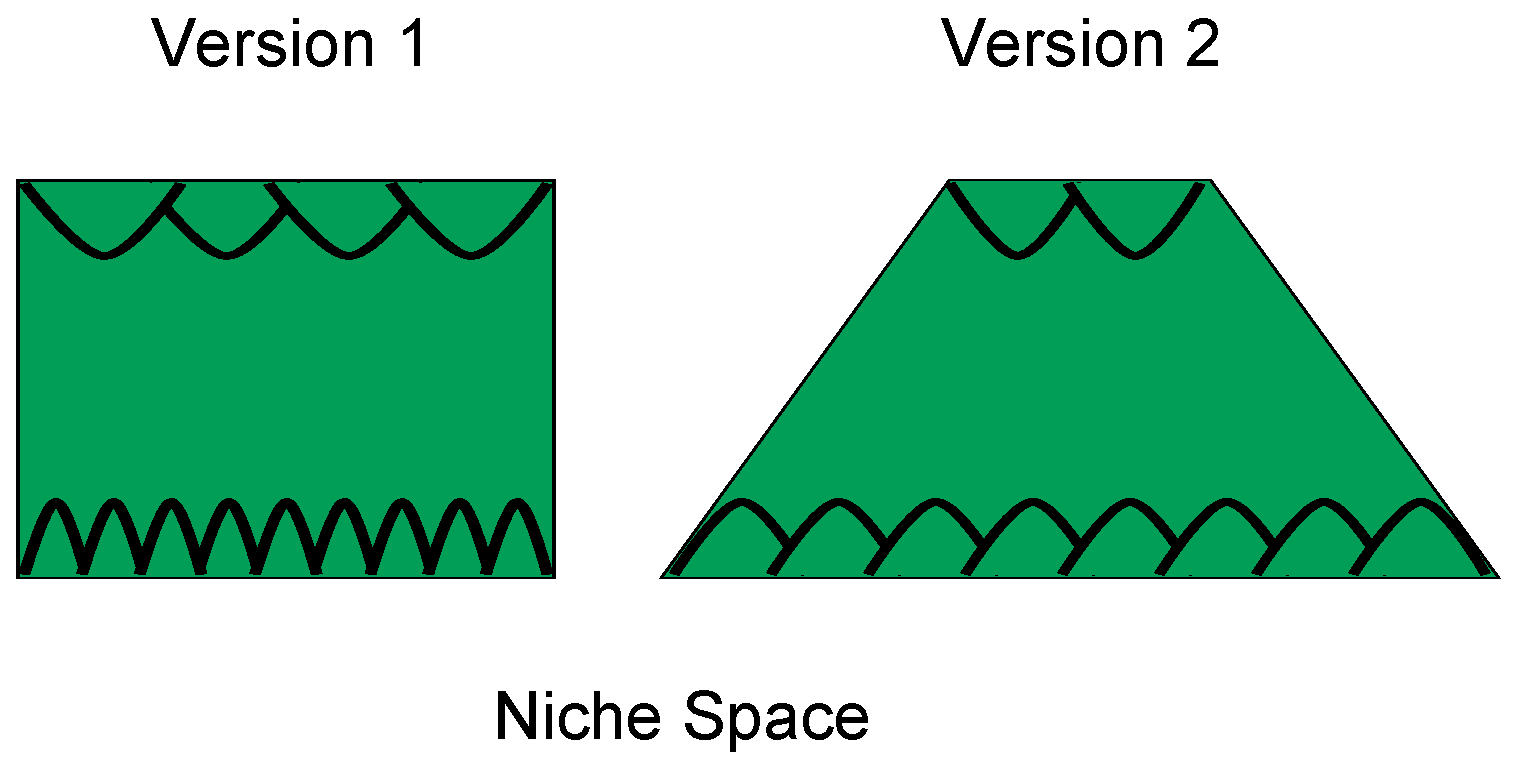
\includegraphics[width=.8\textwidth]{Figures/hypothesis_comparison.eps}

    \end{center}

    \begin{columns}
    \column{.5in}
    \column{1.75in}
      - More feeding links per species in tropics
    \column{.5in}
    \column{1.75in}
      - Similar feeding links per species at all latitudes
    \column{.5in}
    \end{columns}

  \end{frame}


  \begin{frame}{Testing The Hypotheses}

    \begin{center}
      \includegraphics*[width=.8\textwidth]{Figures/LittleRockLake.eps}


    195 food webs \\
    0-78 degrees (absolute latitude) \\
    Mean L/S, Generality, Vulnerability

    \end{center}

  \end{frame}


  \begin{frame}{Testing The Hypotheses}

    \begin{center}
      \includegraphics*[width=.8\textwidth]{Figures/LittleRockLake.eps}


    195 food webs \\
    0-78 degrees (absolute latitude) \\
    Mean \textbf{L/S}, Generality, Vulnerability

    \end{center}

  \end{frame}


\end{document}